\clearpage
\section[Compresión nonádica y momentos circulares de la forma de Weil]{Compresión nonádica y\\momentos circulares de la forma de Weil}
\label{sec:transporte-momentos}
\label{tm-add-seccion}

La relación entre memoria y positividad requiere conservar dos niveles de lectura.
La vuelta nonádica registra una historia y admite una realización hilbertiana
positiva; los lectores aritméticos de esa misma genealogía expresan una forma
hermítica en la que intervienen conjuntamente los canales gamma, primo y polar.
El problema de transporte consiste en identificar sus energías y sus correlaciones,
con los mismos dominios y sin sustituir una de esas realizaciones por la otra.
Las identidades siguientes hacen explícita esa comparación antes de aplicar
la construcción de Gelfand--Naimark--Segal (GNS) a la forma aritmética.

Se conserva primero el balance completo de una coordenatización de nueve fases, incluida
la eventual variación de norma en la costura. Después se construyen el registro
de pérdidas, sus matrices de momentos y un operador de Cayley que actúa sobre
pruebas exponencialmente decrecientes. La coercividad local puede transportarse
a colecciones enteras de pruebas con colas; el paso a su suma algebraica y al dominio
global exige además las correlaciones mixtas que se precisan más adelante.
Este desarrollo no afirma que la positividad global de Weil quede establecida.

% Procedencia y alcance editorial íntegros de las cabeceras originales:
% # Costura nonádica, balance de memoria y transporte de la positividad
% 
% Desarrollo focal del 11 de septiembre de 2026. No modifica las ediciones PDF entregadas. Procedencia: arquitectura autoral preexistente; formalización reunida de las identidades de compresión, con una extensión explícita al caso en que aún se comprueba la isometría de la costura. No se atribuye prioridad histórica a estas identidades operatorias.
% 
% # Momentos circulares antes de GNS: memoria nonádica y forma aritmética completa
% 
% Nota independiente de investigación matemática, 11 de septiembre de 2026.
% No modifica un PDF, un índice ni un certificado de publicación. El resultado
% propio es la composición explícita de dos construcciones anteriores a GNS:
% un núcleo positivo de memoria y unos momentos circulares de la forma completa.
% Su identificación no se presupone.
% 

% SOURCE c L5-20
\subsection{Estado enriquecido y modos de la coordenatización central}
\label{tm-add-c1}
La construcción que se utiliza es APP → TRIT → TPK → estado enriquecido → estructura discreta conjunta del continuo. APP conserva sobre el mismo soporte las evaluaciones de suma y producto, sus cocientes y residuos. El TRIT conserva orientación y régimen; el TPK compone selección, transporte y actualización de memoria. La holonomía nonádica devuelve la fase y aumenta la profundidad de la historia. Los cinco aspectos correlativos del continuo no se separan ni se redefinen mediante la cuestión espectral que se estudia después.

Este desarrollo comienza en la realización del registro de vueltas de esa estructura. No pretende sustituir la construcción completa del continuo por un espacio de sucesiones. La memoria entera es una coordenada del estado, no su totalidad. Tampoco identifica el registro de fase reducido con el generador TPK.

El apunte autoral sobre suma y producto señala la procedencia de la matriz central. En la coordenatización positiva conservada se obtiene

\[
B_c=\begin{pmatrix}7&2\\2&7\end{pmatrix}
=9P_++5P_-,\qquad
P_\pm=\frac12\begin{pmatrix}1&\pm1\\\pm1&1\end{pmatrix}.
\]
Así, después de normalizar el modo uniforme, el modo diferencial tiene razón \(q=5/9\). Los nombres «suma» y «producto» describen las operaciones APP que generan la coordenatización; los proyectores \(P_+\) y \(P_-\) son sus modos simétrico y antisimétrico. La igualdad entre un modo y una hoja concreta necesita conservar el mapa que los relaciona.


% SOURCE c L21-70
\subsection{Compresión uniforme de la coordenatización nonádica y balance exacto}
\label{tm-add-c2}
Sea \(\mathcal K\) un espacio de Hilbert y sea \(C\) un operador acotado sobre él. En \(\mathcal K^9\), la coordenatización de nueve fases con costura \(C\) actúa por

\[
S_C(v_0,\ldots,v_8)=(Cv_8,v_0,\ldots,v_7),
\qquad S_C^9=I_9\otimes C.
\]
La inclusión uniforme es

\[
Jv=\frac13(v,\ldots,v),\qquad J^*J=I.
\]
Escribimos la compresión visible y su componente complementaria como

\[
T=J^*S_CJ=\frac{8I+C}{9},\qquad
\eta=(I-JJ^*)S_CJ.
\]
\begin{proposition}[Balance exacto de la compresión y de la costura]
\label{tm-add-proposicion-costura-1}
Sin suponer que \(C\) sea isométrico, se cumplen

\[
\eta^*\eta=\frac8{81}(I-C)^*(I-C),
\]
\begin{equation}
\boxed{I-T^*T=\eta^*\eta+\frac19(I-C^*C).}
\label{tm-add-balance-costura}
\end{equation}
\end{proposition}

\begin{proof}
La ortogonalidad de \(JJ^*\) da

\[
\eta^*\eta=J^*S_C^*S_CJ-T^*T.
\]
El primer término es \((8I+C^*C)/9\). El segundo es \((64I+8C+8C^*+C^*C)/81\). La resta prueba la primera identidad. Restar ahora \(T^*T\) a \(I\) y separar \(I-(8I+C^*C)/9\) prueba \eqref{tm-add-balance-costura}.
\end{proof}

La fórmula no elimina memoria: muestra exactamente dos contribuciones. Una mide la dispersión entre las nueve fases; la otra mide el defecto de norma de la costura. Si la construcción previa ha dado \(C^*C=I\), queda la identidad positiva de compresión–expresión del corpus:

\[
I-T^*T=\eta^*\eta\succeq0.
\]
Este resultado explica qué contiene la positividad de la memoria y dónde debe intervenir la identificación del lector. No permite reemplazar esa identificación por el dibujo de una circunferencia.


% SOURCE c L71-103
\subsection{Contracción visible y conservación del registro de vueltas}
\label{tm-add-c3}
Supóngase ahora que \(C\) es unitario, como sucede para el desplazamiento bilateral de la memoria entera. La vuelta completa del modo diferencial se representa por \(M=qC\), no por nueve aplicaciones sucesivas del mismo factor \(q\).

Para cada entero \(N\geq1\), se define el registro de pérdidas y terminal

\[
L_Nv=\bigl(\sqrt{1-q^2}v,
\sqrt{1-q^2}qCv,\ldots,
\sqrt{1-q^2}q^{N-1}C^{N-1}v, q^NC^Nv\bigr).
\]
\begin{proposition}[Conservación isométrica del registro de vueltas]
\label{tm-add-proposicion-costura-2}
\(L_N\) es isométrico. Al aumentar \(N\), el último componente se descompone en una nueva memoria expresada y un nuevo terminal, sin borrar el registro anterior. El registro infinito

\[
Lv=\left(\sqrt{1-q^2}q^jC^jv\right)_{j\geq0}
\]
también es isométrico.
\end{proposition}

\begin{proof}
Para \(v,w\in\mathcal K\),

\[
\langle L_Nv,L_Nw\rangle
=\left[(1-q^2)\sum_{j=0}^{N-1}q^{2j}+q^{2N}\right]
\langle v,w\rangle=\langle v,w\rangle.
\]
En el último componente, \(q^NC^Nv\) se transforma en \((\sqrt{1-q^2}q^NC^Nv,q^{N+1}C^{N+1}v)\); esa transformación conserva el producto interior. El terminal tiene norma \(q^N\|v\|\), que tiende a cero; la suma infinita converge y conserva la norma.
\end{proof}

Para dos estados iniciales, esta prueba conserva sus productos cruzados; no consiste sólo en sumar energías de trayectorias aisladas. El signo positivo de la memoria procede de la ortogonalidad de sus residencias y de la isometría del transporte que ya se ha construido.


% SOURCE c L104-111
\subsection{Círculo dual de memoria y coordenatización aritmética de Cayley}
\label{tm-add-c4}
El registro entero de vueltas admite el desplazamiento bilateral \(Se_n=e_{n+1}\) sobre \(\ell^2(\mathbb Z)\). Sus caracteres \(n\mapsto z^n\), \(|z|=1\), dan el círculo dual de la memoria. La fase visible \(r\in\{0,\ldots,8\}\) retorna; el entero \(n\) no se reduce módulo \(12\) en el estado completo.

Si se impone esa reducción, un carácter sólo desciende cuando \(z^{12}=1\). Por tanto, la memoria sin reinicio tiene una consecuencia precisa: permite el círculo completo de caracteres, mientras que el calendario finito sólo conserva una selección finita. No se deduce de ello qué medida aritmética se realiza sobre ese círculo.

El segundo círculo que aparece en el capítulo espectral del integral es una coordenatización de la realización de Cayley. La subsección~\ref{tm-add-m4} construye un operador de Cayley directamente sobre las funciones de prueba antes de construir un espacio de Hilbert mediante la forma de Weil. Así se puede comparar el transporte aritmético con el de memoria sin introducir las alturas de los ceros como entradas.


% SOURCE c L112-163
\subsubsection{Conservación de la forma aritmética bajo compresión nonádica}
\label{tm-add-c4-1}
La invariancia aritmética del lector de Cayley auxiliar permite una composición adicional. Para \(a>b>1/2\), sea \(C_a\) el operador construido en la subsección~\ref{tm-add-m4} y sea \(\mathcal T_a=(8I+C_a)/9\). La igualdad \(\mathscr W(C_af,C_ag)=\mathscr W(f,g)\) implica, por expansión,

\begin{equation}
\boxed{\mathscr W(f,g)=\mathscr W(\mathcal T_af,\mathcal T_ag)
+\frac8{81}\mathscr W((I-C_a)f,(I-C_a)g).}
\label{tm-add-balance-aritmetico}
\end{equation}
Esta identidad conserva el canal gamma, los relojes primos y el término polar conjuntamente. No presupone que la forma sea positiva. El cálculo consiste en sumar los coeficientes: los términos mixtos tienen coeficientes \(8\) y \(-8\), que se cancelan, mientras que los dos términos diagonales aportan \(72+9=81\) veces la forma inicial. Su iteración finita da

\begin{equation}
\mathscr W(f,g)=\mathscr W(\mathcal T_a^Nf,\mathcal T_a^Ng)
+\frac8{81}\sum_{j=0}^{N-1}
\mathscr W((I-C_a)\mathcal T_a^jf,(I-C_a)\mathcal T_a^jg).
\label{tm-add-balance-iterado}
\end{equation}
En la representación ordinaria \(L^2\), donde \(C_a\) ya es unitario, el mismo cálculo es una descomposición positiva de norma. Sobre la forma aritmética es, inicialmente, una conservación exacta de energía firmada. La diferencia entre esas dos afirmaciones queda situada en una identidad común; no se oculta en un cambio de representación.

En una coordenatización circular \(z=e^{i\theta}\), la compresión envía \(z\) a \(t(z)=(8+z)/9\). Por tanto,

\[
1-|t(z)|^2=\frac8{81}|1-z|^2
=\frac{32}{81}\sin^2(\theta/2).
\]
La separación angular tiene así una expresión exacta como energía complementaria. Ésta es la imagen de la compresión nonádica de una coordenatización de fase; no se identifica por el dibujo con otro operador del corpus. Tampoco se confunde este mapa \(t(z)\) con el factor radial \(5/9\), que procede de los dos modos de la coordenatización APP central.

\begin{figure}[htbp]
\centering
\begin{tikzpicture}[font=\small,>=stealth]
\begin{scope}[x=1cm,y=1cm]
\draw[->,gray] (-2.35,0)--(2.65,0) node[right] {$\Re z$};
\draw[->,gray] (0,-2.2)--(0,2.25) node[above] {$\Im z$};
\draw[thick] (0,0) circle (2);
\draw[very thick] (1.777778,0) circle (.222222);
\fill (1,1.732051) circle (1.5pt) node[above right] {$z$};
\fill (1.888889,.19245) circle (1.5pt);
\draw[->] (1.10,1.57)--(1.85,.34);
\draw[dotted] (0,0)--(1,1.732051);
\draw (1.95,.20)--(2.65,.75) node[right] {$t(z)$};
\node[below] at (2,0) {$1$};
\node[above left] at (-1.30,1.4) {$|z|=1$};
\node[align=center] at (0,-2.72)
 {$t(z)=\dfrac{8+z}{9}$\\[3pt]
 $\left|t(z)-\dfrac89\right|=\dfrac19$};
\end{scope}
\begin{scope}[shift={(8,0)}]
\node[align=center] (f) at (0,1.5) {Representación de fase\\[3pt] $r\longmapsto r$};
\node[align=center] (m) at (0,0) {Transporte de memoria\\[3pt] $(r,n)\longmapsto(r,n+1)$};
\draw[->,thick] (f)--(m);
\node[draw,rounded corners,inner sep=8pt,align=center] at (0,-1.65)
 {$1-|t(z)|^2=\dfrac8{81}|1-z|^2$\\[5pt]
 Representación y complemento};
\end{scope}
\end{tikzpicture}
\caption{La coordenatización circular de la compresión nonádica. A la izquierda,
el círculo unidad y su imagen de centro \(8/9\) y radio \(1/9\),
dibujados a la misma escala; se muestra la imagen de \(z=e^{i\pi/3}\).
A la derecha, el retorno de fase se acompaña de avance de memoria.
El balance inferior cuantifica la componente complementaria. Esta figura
representa el mapa \(t\), distinto del factor modal \(q=5/9\) de la
coordenatización central.}
\label{fig:compresion-circular}
\end{figure}


El desarrollo local de Schur da signo positivo a la forma aritmética en un dominio funcional concreto y a sus imágenes por transporte. Las identidades \eqref{tm-add-balance-aritmetico}–\eqref{tm-add-balance-iterado} no autorizan por sí solas a declarar positivos todos sus sumandos para una prueba arbitraria: permiten localizar exactamente qué energías y correlaciones debe conservar una extensión de ese dominio.


% SOURCE c L164-190
\subsection{Criterio de transporte de positividad mediante momentos mixtos}
\label{tm-add-c5}
Sea \(\mathcal D\) el dominio común de los lectores previamente construidos. Sea \(\mathscr W\) la forma sesquilineal que expresan sus canales gamma, primos y polar. La fórmula analítica se recibe después del generador nativo; no selecciona las semillas ni los coeficientes anteriores.

Sean \(C_a\) el transporte reversible sobre pruebas y \(S\) el desplazamiento de la memoria. Se utiliza explícitamente \(C_a(\mathcal D)=\mathcal D\) y la identidad \(\mathscr W(C_af,C_ag)=\mathscr W(f,g)\), demostrada para la clase exponencial de pruebas en las subsecciones~\ref{tm-add-m4} y~\ref{tm-add-m5}. Para una colección \(\mathcal E\subset\mathcal D\), supóngase construido un mapa lineal \(V:\operatorname{span}\mathcal E\to\mathcal K\) tal que, para todo \(f,g\) de esa colección y todo entero \(n\),

\begin{equation}
\boxed{\mathscr W(C_a^n f,g)=\langle S^nVf,Vg\rangle.}
\label{tm-add-criterio-momentos}
\end{equation}
\begin{proposition}[Transporte de positividad por identificación de momentos]
\label{tm-add-proposicion-costura-3}
La identidad \eqref{tm-add-criterio-momentos} implica la positividad de \(\mathscr W\) sobre el espacio generado por las órbitas \(C_a^n\mathcal E\). Si ese espacio es denso en \(\mathcal D\) para la norma conjunta de los lectores, y éstos son continuos para esa norma, la positividad se extiende a \(\mathcal D\).
\end{proposition}

\begin{proof}
Para \(F=\sum_j C_a^{n_j}f_j\), la invariancia de \(\mathscr W\) bajo \(C_a\) y \eqref{tm-add-criterio-momentos} dan

\[
\begin{aligned}
\mathscr W(F,F)
&=\sum_{i,j}\mathscr W(C_a^{n_i-n_j}f_i,f_j)\\
&=\left\|\sum_i S^{n_i}Vf_i\right\|^2\geq0.
\end{aligned}
\]
Si una combinación representa la función cero, la misma identidad fuerza que la combinación de vectores tenga norma cero; la realización queda bien definida. El paso a la clausura usa la continuidad de los dos lectores, no una elección posterior del signo.
\end{proof}

Éste es un criterio de construcción con dominios explícitos, no una afirmación de que \eqref{tm-add-criterio-momentos} haya sido demostrada para todos los lectores del corpus. Para extender desde la colección inicial a sus órbitas hay que conservar todos los momentos cruzados: demostrarlo sólo con \(n=0\) sobre esa colección inicial no completa dicha extensión. Naturalmente, una identidad de Gram ya demostrada para \(n=0\) sobre todo \(\mathcal D\) probaría directamente la positividad en ese dominio.


% SOURCE c L191-211
\subsection{Identificación de energía y realización por dos columnas}
\label{tm-add-c6}
El corpus conserva dos columnas \(J_+\) y \(J_-\) y un conector analítico efectivo entre ellas. También describe una codificación nativa \(\Xi\) y una proyección ortogonal \(P\). Cuando las dos identidades de momentos se calculan en el mismo dominio,

\[
\langle\Xi f,\Xi g\rangle=\langle J_+f,J_+g\rangle,
\qquad
\langle P\Xi f,P\Xi g\rangle=\langle J_-f,J_-g\rangle,
\]
la resta da

\begin{equation}
\mathscr W(f,g)=\langle(I-P)\Xi f,(I-P)\Xi g\rangle.
\label{tm-add-dos-columnas}
\end{equation}
El expediente calcula la expectativa uniforme y el refinamiento de Helmert por separado. Su conjugación conjunta conserva los dos Grams y no puede, por un mero cambio de notación, convertir un operador de diferencia en uno de evaluación. El conector gamma recuperado realiza una operación analítica adicional, que debe conservar su presupuesto de energía. Esta precisión reúne las operaciones existentes; no declara inexistente la arquitectura del TPK.

Las fórmulas \eqref{tm-add-criterio-momentos} y \eqref{tm-add-dos-columnas} son dos expresiones compatibles de la vía que se quiere completar: la primera organiza los retornos y sus correlaciones, la segunda organiza la parte visible y la memoria complementaria. La estimación por complemento de Schur del expediente da un control efectivo de esa energía en una ventana completa y en todos sus refinamientos. Su alcance se declara con la ventana concreta, sin sustituir con ella el dominio global.


% BEGIN PROCEDENCIA COSTURA, FUENTE L212
% ## 7. Localizadores materiales y continuidad
% 
% - APP central, modos \(9/5\): `base_c01_sin_encabezado.tex`, construcción de la carta central; capítulo `78_doble_circulo_campo_espectral_completo.tex`, entorno de líneas 1276–1280.
% - Memoria anterior a la representación espectral: `cap08_holonomia_helice_memoria.tex`, especialmente la cubierta entera y la publicación \(C_{108}\).
% - Conexión y compresión–expresión: `certificados/ley_nueve_puertas_2026-07-30/DELTA_CONEXION_NONADICA_CONJUNTA_COMPRESION_EXPRESION_2026-08-16.md`, §§1–3.
% - Doble círculo y transporte cilíndrico: propietario `78_doble_circulo_campo_espectral_completo.tex`, líneas 940–1260.
% - Dos momentos nativos: propietario `10b_prueba_espectral_polar_riemann_weil_rectificacion_probatoria_20260903.tex`, líneas 235–452.
% - Propietarios completos y rutas absolutas: [recuperación conservada](../ARITMETICA_GENEALOGICA_PRIMOS_DESARROLLO_DOBLE_CIRCULO_20260911/01_HALLAZGOS_PROPIETARIOS_DOBLE_CIRCULO.md).
% 
% La selección editorial sigue siendo el integral de 2.249 páginas y sus desarrollos adyacentes. Los verificadores históricos que devuelven 2.084 páginas no cambian esa selección. Ningún control de huellas o de compilación se utiliza aquí como prueba de positividad global.
% END PROCEDENCIA COSTURA

% SOURCE m L9-53
\subsection{Procedencia operatoria y función de los lectores}
\label{tm-add-m1}

% BEGIN LOCALIZADORES M1
% Propietarios y localizadores de esta lectura:
% 
% - Integral autoral de 2.249 páginas, propietario
%   `output/REVISION_EDITORIAL_HMT_MD_20260905/01_FUENTES/INTEGRAL/tree/New project/output/ENSAMBLADO_CAUSAL_RESTAURADO_HMT_MD_20260905/fuente/manuscrito/integracion_83/parte_v/tex/fuentes_propietarias/editor_ready/78_doble_circulo_campo_espectral_completo.tex`.
%   Se ha releído su cuerpo completo, 1–1929, en la copia conservada en el
%   manuscrito de primos. El cociclo está en 943–968; el orden
%   positividad → GNS → Stone → Cayley, en 525–612 y 969–987; el transporte
%   cilíndrico torcido, en 1023–1118; la pérdida por vuelta, en 1171–1237;
%   la costura de nueve fases, en 1421–1495; la fórmula aritmética, en 1578–1610.
% - `output/ARITMETICA_GENEALOGICA_PRIMOS_DESARROLLO_DOBLE_CIRCULO_20260911/01_HALLAZGOS_PROPIETARIOS_DOBLE_CIRCULO.md`, leído completo. Conserva los
%   localizadores de los antecedentes del bloque APP y de la memoria anteriores
%   al GNS; no se confunde su lectura con una nueva lectura íntegra de cada
%   antecedente que cita.
% - `output/ARITMETICA_GENEALOGICA_PRIMOS_PRESENTACION_20260911/antecedentes/recuperacion_gamma/narrativa_205_paginas/CONSTANTES_ESTRUCTURA_Y_REALIDAD_FISICA_RECOPILACION_INTEGRA.md`, lectura focal 5710–5905. En 5740–5869 reúne producto nativo,
%   irreducibles, ocupaciones, calor/Mellin, canal polar y los dos círculos.
%   No ofrece allí una secuencia Toeplitz adicional anterior a GNS.
% - `output/ARITMETICA_GENEALOGICA_PRIMOS_PRESENTACION_20260911/manuscrito/03_DOBLE_CIRCULO_Y_TRANSPORTE_ESPECTRAL.md`, §§2–3, para la forma completa,
%   su continuidad y las dos columnas; en este corte se ha releído §2,
%   líneas 119–191, y se conserva el análisis anterior de §3.
% - `output/AUDITORIA_INTEGRAL_PUBLICABILIDAD_HMT_MD_20260906/COORDINACION_20260906/TRAZA_GENERATIVA_COORDINADA.md`: consulta focal de lectores espectrales;
%   desde 1524 remite a los momentos primos, no a una medida circular de Weil
%   ya seleccionada por la memoria.
% 
% La puerta del núcleo permanente y su autocomprobación causal pasaron. La
% puerta histórica `apply-hmt-first-principles` resuelve 2.084 páginas; se conserva
% como control de ese testigo, no como sustituto de la selección autoral de
% 2.249 páginas. No se afirma lectura íntegra del corpus ni del documento de 205
% páginas.
% 
% END LOCALIZADORES M1
La cadena utilizada es APP → TRIT → TPK → historias enriquecidas del continuo conjunto → lectores aritméticos y de memoria → representación circular. Las cinco operaciones del continuo permanecen sobre las mismas historias; este desarrollo estudia un lector de su memoria, no construye una quinta rama aislada. La lectura prima usa los irreducibles producidos por el producto nativo; las constantes ya expresadas por HMT intervienen sólo después en los lectores.

\textbf{Procedencia.} Cociclo, pérdida, dos hojas, grupos de memoria y doble círculo: arquitectura autoral preexistente y resultados recuperados. Las pruebas reunidas que siguen son una formalización nueva de estos antecedentes. No se reivindica prioridad histórica de los núcleos de Poisson, de Cayley ni de las identidades Toeplitz. La procedencia de esta composición exacta dentro del corpus no ha sido agotada fuera de los propietarios indicados.


% SOURCE m L54-83
\subsection{Representación regular de memoria anterior al GNS aritmético}
\label{tm-add-m2}
El bloque central de APP, con sus proyectores simétrico y antisimétrico, es

\[
B_c=\begin{pmatrix}7&2\\2&7\end{pmatrix}
=9P_++5P_-.
\]
La normalización del modo diferencial expresa \(q=5/9\). La vuelta completa del TPK conserva la fase e incrementa la memoria entera:

\[
m(\Gamma_9^n)=n,\qquad
m(\gamma_2\gamma_1)=m(\gamma_2)+m(\gamma_1).
\]
Sobre una órbita reversible de esa memoria, sus estados levantados se identifican con \(e_n\), \(n\in\mathbb Z\), y la vuelta es el desplazamiento \(Se_n=e_{n+1}\). La inyectividad de esa enumeración procede del incremento de memoria. Si se parte sólo del semigrupo de vueltas positivas, el mismo espacio bilateral es la extensión de desplazamiento que añade sus antecedentes; no se atribuye reversibilidad a una transición que sólo se haya demostrado isométrica. En un árbol completo se conservan las restantes etiquetas en un factor transversal: el desplazamiento actúa sobre memoria, no identifica rutas.

Este \(S\) no es el Cayley de Weil insertado en la costura. Es la realización regular de la operación entera de memoria. Su positividad hilbertiana se conoce antes de formar un GNS de la forma aritmética.


% SOURCE m L84-120
\subsubsection{Vector de pérdidas, correlaciones y término terminal}
\label{tm-add-m2-1}
La telescopía por vueltas produce pesos \((1-q^2)q^{2j}\). Su amplitud en la memoria es el vector explícito

\[
v_q=\sqrt{1-q^2}\sum_{j=0}^{\infty}q^j e_j,
\qquad \|v_q\|^2=1.
\]
Con producto interior lineal en la primera variable, para \(n\ge0\),

\[
\langle S^n v_q,v_q\rangle
=(1-q^2)\sum_{j\ge0}q^j q^{j+n}=q^n.
\]
La conjugación y la unitariedad dan, para todo entero,

\[
\boxed{m_n^{\mathrm{mem}}=q^{|n|}.}
\]
El truncamiento \(v_{q,N}=\sqrt{1-q^2}\sum_{j=0}^{N-1}q^j e_j\) conserva exactamente el terminal:

\[
\|v_{q,N}\|^2=1-q^{2N},\qquad
\langle S^n v_{q,N},v_{q,N}\rangle
=q^n\bigl(1-q^{2(N-n)}\bigr),\quad 0\le n<N.
\]
Para \(n\ge N\), esa correlación truncada vale cero. Por tanto, para cada \(n\) fijo, la diferencia respecto del momento completo es \(q^{2N-n}\) cuando \(N>n\), y tiende a cero. Esta fórmula no borra el último registro ni equipara un truncamiento con toda la historia.


% SOURCE m L121-159
\subsubsection{Factorización triangular y determinante de las matrices de memoria}
\label{tm-add-m2-2}
Para índices \(0,\ldots,N\), defínase

\[
T_N=(q^{|i-j|})_{0\le i,j\le N}.
\]
Es un Gram de \(v_q,Sv_q,\ldots,S^Nv_q\), de modo que

\[
\sum_{i,j=0}^{N}\overline{c_i}c_j(T_N)_{ij}
=\left\|\sum_{j=0}^{N}c_jS^jv_q\right\|^2\ge0.
\]
Hay además una prueba exacta sin series infinitas. Sean

\[
L_{ij}=\begin{cases}q^{i-j},&i\ge j,\\0,&i<j,\end{cases}
\qquad D=\operatorname{diag}(1,1-q^2,\ldots,1-q^2).
\]
Entonces \(T_N=LDL^*\). Para \(i\ge j\), la entrada del producto es

\[
q^{i+j}+(1-q^2)\sum_{k=1}^{j}q^{i+j-2k}
=q^{i-j}.
\]
Por simetría se obtiene la identidad entera de matrices. Una Cholesky es \(L D^{1/2}\), y, puesto que \(\det L=1\),

\[
\boxed{\det T_N=(1-q^2)^N=(56/81)^N>0.}
\]
Este núcleo positivo nace de la pérdida y de la memoria conservada. No requiere ceros, una función zeta positiva ni un GNS de Weil.


% SOURCE m L160-184
\subsection{Fase, refinamiento nonádico y convergencia débil de estados}
\label{tm-add-m3}
Una representación por fase fija se obtiene de

\[
v_{r,\theta}=\sqrt{1-r^2}\sum_{j\ge0}r^j e^{-ij\theta}e_j,
\quad 0<r<1,
\]
y produce \(m_n=r^{|n|}e^{in\theta}\). Las Toeplitz son conjugadas diagonalmente de las anteriores y tienen determinante \((1-r^2)^N\). La fase \(\theta\) es aquí una coordenada de la colección de caracteres; no se ha seleccionado una fase espectral aritmética.

Sobre el círculo, con Haar normalizada \(d\lambda\), esos momentos poseen la medida explícita

\[
d\nu_{r,\theta}(z)
=\frac{1-r^2}{|1-r e^{-i\theta}z|^2}\,d\lambda(z).
\]
La expansión de ambas series geométricas prueba directamente sus coeficientes de Fourier, sin usar una medida objetivo.


% SOURCE m L185-219
\subsubsection{Raíces nonádicas del radio y compatibilidad de fases}
\label{tm-add-m3-1}
Tomando \(r_m=q^{1/9^m}\), se cumple \(0<r_m<1\), \(r_{m+1}^{9}=r_m\) y \(r_m\to1\). Para fase fija,

\[
r_m^{|n|}e^{in\theta}\longrightarrow e^{in\theta}
\quad\text{para cada }n\in\mathbb Z.
\]
Las medidas son probabilidades; la aproximación uniforme por polinomios trigonométricos extiende la convergencia de los momentos a toda función continua. En consecuencia,

\[
\nu_{r_m,\theta}\ \rightharpoonup\ \delta_{e^{i\theta}}.
\]
Esto muestra cómo una medida atómica puede surgir como límite débil de estados de memoria. No es un límite fuerte de los vectores en la misma representación regular: cada coeficiente de \(v_{r_m,\theta}\) tiende a cero, pero sus normas siguen siendo uno.

Hay que conservar una precisión de naturalidad. Bajo \(p_9(z)=z^9\),

\[
(p_9)_*\nu_{r,\theta}=\nu_{r^9,9\theta}.
\]
Por tanto, el radio nonádico con fase fija \textbf{no} da por sí solo un sistema proyectivo de medidas bajo \(p_9\). Para ello deben conservarse fases levantadas con \(9\theta_{m+1}=\theta_m\pmod{2\pi}\), incluidas sus elecciones de rama; o bien declararse que el refinamiento usado mantiene la coordenada angular y sólo cambia el radio. Son operaciones distintas.


% SOURCE m L220-236
\subsubsection{Selección del estado y cambio de tipo espectral}
\label{tm-add-m3-2}
La memoria produce el grupo, la positividad de sus Grams y estas colecciones compatibles de correlación. Una fase concreta o una mezcla de fases exige el lector que selecciona sus amplitudes. Por ejemplo, el vector \(e_0\) produce \(m_n=\mathbf1_{n=0}\); \((e_0+e_1)/\sqrt2\) produce \(m_0=1,m_{\pm1}=1/2\) y los demás momentos nulos. La misma operación de memoria admite ambos estados positivos.

La representación regular tiene medidas vectoriales absolutamente continuas respecto de Haar. Un filtro vectorial \(L^2\) fijo no puede producir una medida puramente atómica no nula. El límite débil anterior muestra una vía precisa para que cambie el tipo espectral al refinar: hay que conservar y controlar ese límite de estados, no sólo aumentar la longitud de una órbita de fase previamente elegida. Esto no niega la representación espectral del corpus ni la generación conjunta HMT; distingue los dominios de dos lectores.


% SOURCE m L237-295
\subsection{Operador de Cayley sobre el dominio exponencial de pruebas}
\label{tm-add-m4}
Ahora se construye un segundo objeto, sin suponer positividad de Weil. El producto nativo y sus irreducibles ya proporcionan \(\ell_{p,k}=k\log p\), \(w_{p,k}=(\log p)p^{-k/2}\). Las lecturas gamma y polar completan la forma \(\mathscr W\) escrita en la subsección~\ref{tm-add-m5}. El papel de la memoria es ofrecer un índice entero de iteración; el operador siguiente actúa efectivamente sobre las funciones de esa representación.

El operador \(C_a\) es un lector analítico auxiliar de esta formalización. La elección \(a>1/2\) no reemplaza silenciosamente la costura canónica \(a=1/2\), ni se declara que esa elección haya sido ya seleccionada por el TPK.

Fíjense \(a>b>1/2\). Sea \(\mathscr E_b\) el espacio de funciones suaves tales que, para cada derivada de orden \(j\), \(\sup_x e^{b|x|}|f^{(j)}(x)|<\infty\). Contiene todas las pruebas compactamente soportadas. Defínanse

\[
(R_a^+f)(x)=\int_0^\infty e^{-at}f(x+t)\,dt,
\qquad
(R_a^-f)(x)=\int_0^\infty e^{-at}f(x-t)\,dt,
\]
\[
\boxed{C_af=f-2aR_a^+f,\qquad C_a^{-1}f=f-2aR_a^-f.}
\]
Estas integrales son lectores de traslación construidos sobre las pruebas; no utilizan el espectro de los ceros. El parámetro \(a=1\), por ejemplo, procede de la unidad y deja elegir \(1/2<b<1\); no calibra ningún cero.

\paragraph{Dominio, inversa y realización unitaria.} La desigualdad \(e^{b|x|}|f(x\pm t)|\le M_0e^{bt}\) da la cota \(\|R_a^\pm f\|_b\le\|f\|_b/(a-b)\), también para cada derivada. Así, ambos operadores preservan \(\mathscr E_b\). Con la convención \(\widehat f(z)=\int f(x)e^{-izx}\,dx\), sus multiplicadores son

\[
\widehat{C_af}(z)=c_a(z)\widehat f(z),\qquad
c_a(z)=\frac{z-ia}{z+ia},
\]
y el multiplicador del operador inverso es \(c_a(z)^{-1}\). La identidad en Fourier real prueba ambas composiciones inversas. En \(L^2\), \(|c_a(t)|=1\), de modo que \(C_a\) es unitario para la norma ordinaria, sin utilizar la norma de Weil. Sobre pruebas puede escribirse \(C_a=(H+ia)(H-ia)^{-1}\) con \(H=i\partial_x\); aquí la fórmula integral, no un generador GNS, define los operadores.

\paragraph{Condición de convergencia en el borde polar.} El parámetro \(a=1/2\) del Cayley del propietario no puede introducirse sin más en estas integrales pre-GNS. Para una prueba compacta, \(R_{1/2}^+f\) tiene en general una cola proporcional a \(e^{x/2}\) hacia \(-\infty\); su evaluación polar negativa no converge. No se ha probado una divergencia de la forma reunida, sino que esta descomposición término a término exige el margen \(a>1/2\). El Cayley del GNS puede usar después \(a=1/2\) sobre su dominio hilbertiano.


% SOURCE m L296-352
\subsection{Conservación conjunta de los canales gamma, primo y polar}
\label{tm-add-m5}
Para \(f,g\in\mathscr E_b\), sean

\[
C_{f,g}(u)=\int f(x)\overline{g(x-u)}\,dx,
\qquad P_f^\pm=\int f(x)e^{\pm x/2}\,dx.
\]
La forma completa se define por

\[
\begin{aligned}
\mathscr W(f,g)={}&c_\Gamma C_{f,g}(0)
+\int_0^\infty\frac{e^{-u/2}}{1-e^{-2u}}
 [2C_{f,g}(0)-C_{f,g}(u)-C_{f,g}(-u)]\,du\\
&-\sum_{p,k}w_{p,k}
 [C_{f,g}(\ell_{p,k})+C_{f,g}(-\ell_{p,k})]\\
&+P_f^+\overline{P_g^-}+P_f^-\overline{P_g^+},
\qquad c_\Gamma=\psi(1/4)-\log\pi.
\end{aligned}
\]
\paragraph{Existencia y continuidad de la forma completa.} La cota de correlación \(|C_{f,g}(u)|\le M_fM_g(|u|+1/b)e^{-b|u|}\) prueba la convergencia absoluta de la suma prima, dominada por una serie del tipo \(\sum_{n\ge2}(\log n)(1+\log n)n^{-b-1/2}\). La diferencia simétrica de correlaciones es \(O(u^2)\) en cero, mientras el peso gamma es \(O(u^{-1})\); en infinito el peso es exponencial. Las evaluaciones polares convergen porque \(b>1/2\). Estas cotas prueban también la continuidad en los seminormas indicados. No se usa positividad.

\paragraph{Invariancia simultánea de los tres canales.}
\label{tm-add:invariancia-weil} Como \(C_a\) es unitario en \(L^2\) y conmuta con todas las traslaciones,

\[
C_{C_af,C_ag}(u)=C_{f,g}(u)\qquad(u\in\mathbb R).
\]
Por Fubini, los dos lectores polares verifican

\[
P_{C_af}^+=-\frac{a-1/2}{a+1/2}P_f^+,
\qquad
P_{C_af}^-=-\frac{a+1/2}{a-1/2}P_f^-.
\]
Los factores son reales y recíprocos, por lo que cada producto polar cruzado queda exactamente conservado. Reuniendo los tres canales,

\[
\boxed{\mathscr W(C_af,C_ag)=\mathscr W(f,g).}
\]
La identidad vale para todas las potencias enteras y para todos los términos cruzados. Demuestra invariancia de una forma hermítica, no su signo.


% SOURCE m L353-383
\subsection{Momentos circulares de la forma aritmética completa}
\label{tm-add-m6}
Defínanse

\[
m_n^{\mathrm{ar}}(f,g)=\mathscr W(C_a^n f,g),\qquad n\in\mathbb Z.
\]
La fórmula completa de la subsección~\ref{tm-add-m5}, con \(C_a^nf\) en su primera entrada, calcula estos momentos desde primos, gamma y polar. Cada evaluación existe en \(\mathscr E_b\); no requiere una lista de ceros ni una métrica positiva. La hermiticidad y la invariancia anterior dan

\[
m_{-n}^{\mathrm{ar}}(g,f)=\overline{m_n^{\mathrm{ar}}(f,g)},\qquad
\mathscr W(C_a^j f,C_a^k g)=m_{j-k}^{\mathrm{ar}}(f,g).
\]
Para una sola prueba, la matriz \(T_N^{\mathrm{ar}}(f)_{jk}=m_{k-j}^{\mathrm{ar}}(f,f)\) es hermítica Toeplitz y satisface la identidad exacta

\[
c^*T_N^{\mathrm{ar}}(f)c
=\mathscr W\!\left(\sum_{k=0}^N c_k C_a^k f,
                    \sum_{k=0}^N c_k C_a^k f\right).
\]
Se ha construido la matriz sin asumir que sea positiva. La igualdad permite contrastar su positividad con un Gram nativo de memoria; no la presupone.


% SOURCE m L384-406
\subsubsection{Crecimiento polar y condición necesaria de cancelación}
\label{tm-add-m6-1}
Para \(a=1\), la contribución polar exacta a \(m_n^{\mathrm{ar}}(f,g)\) es

\[
(-1/3)^nP_f^+\overline{P_g^-}
+(-3)^nP_f^-\overline{P_g^+}.
\]
Para una prueba real, par y positiva no nula, \(P_f^+=P_f^-=p>0\), de modo que aparece \(p^2[(-1/3)^n+(-3)^n]\). Si el momento total es positivo definido, sus menores de orden dos obligan a

\[
|m_n^{\mathrm{ar}}(f,f)|\le m_0^{\mathrm{ar}}(f,f).
\]
Por ello, la identificación circular debe contabilizar la cancelación concreta de ese crecimiento con los canales gamma y primo. Una simetría formal de las dos hojas no sustituye ese cálculo. Esta observación no declara que la cancelación falle; proporciona un falsador exacto para una candidata a composición.


% SOURCE m L407-424
\subsubsection{Matrices de momentos mixtos y cobertura del dominio}
\label{tm-add-m6-2}
Para una colección de pruebas \(f_1,\ldots,f_d\), el objeto adecuado es el Toeplitz por bloques

\[
\mathsf T_{(j,r),(k,s)}
=m_{k-j}^{\mathrm{ar}}(f_s,f_r).
\]
Su forma cuadrática es \(\mathscr W(F,F)\), donde \(F=\sum_{k,s}c_{k,s}C_a^k f_s\). Controlar sólo las matrices escalares de algunas pruebas no controla los cruces entre pruebas diferentes. Para una colección densa en cada \(C_c^\infty([-R,R])\), la continuidad demostrada permite pasar al dominio completo, siempre que se hayan establecido los Grams mixtos y las compatibilidades al aumentar \(R\). El crecimiento de \(N\) de una única órbita no prueba esa cobertura.


% SOURCE m L425-477
\subsubsection{Transporte de coercividad local a subespacios con colas}
\label{tm-add-m6-3}
\label{tm-add:familias-transportadas}
La identidad anterior tiene una aplicación positiva que no exige identificar todavía todos los momentos con la memoria. Supóngase demostrada por el complemento de Schur, en el intervalo \(I=(-1/18,1/18)\), la cota

\[
\mathscr W(f,f)\geq\tfrac12\|f\|_{L^2}^2,
\qquad f\in C_c^\infty(I).
\]
Este apartado recibe esa estimación como resultado del cálculo local correspondiente; no la deduce de la existencia de \(C_a\). Sea \((\tau_t f)(x)=f(x-t)\). La traslación conserva las correlaciones y satisface

\[
P_{\tau_t f}^{\pm}=e^{\pm t/2}P_f^{\pm}.
\]
Sus productos polares cruzados también se conservan. Por tanto, \(\mathscr W(\tau_t f,\tau_t g)=\mathscr W(f,g)\), y la norma ordinaria \(L^2\) es invariante. Como \(C_a\) y \(\tau_t\) conmutan, para todo entero \(n\), todo \(t\in\mathbb R\) y toda prueba local,

\[
\boxed{\mathscr W(C_a^n\tau_t f,C_a^n\tau_t f)
=\mathscr W(f,f)
\geq\tfrac12\|C_a^n\tau_t f\|_{L^2}^2.}
\]
Para \((n,t)\) fijo, ésta es una cota coerciva en todo el subespacio \(C_a^n\tau_t C_c^\infty(I)\), no sólo en un ejemplo. Cuando \(n\ne0\), las pruebas transformadas pueden tener colas exponenciales no compactas. En su forma aritmética pueden intervenir infinitos relojes primos; la igualdad exacta de los tres canales controla su composición, y las cotas de la subsección~\ref{tm-add-m5} garantizan la convergencia. No se ha sustituido esa suma por un truncamiento finito.

Los términos cruzados entre subespacios con exponentes o traslaciones distintos conservan, en cambio, sus momentos completos. Por ejemplo,

\[
\mathscr W(C_a^n\tau_t f,C_a^m\tau_s g)
=\mathscr W(C_a^{n-m}\tau_{t-s}f,g).
\]
La cota de cada subespacio individual no implica la positividad de su suma algebraica. Ésta se decide mediante los Grams mixtos de la subsección~\ref{tm-add-m6-2}. Así queda aislado un alcance positivo efectivo —colecciones enteras de pruebas con colas— sin promoverlo a todo el dominio por la sola invariancia del transporte.


% SOURCE m L478-521
\subsection{Identificación prospectiva de los momentos y de la energía}
\label{tm-add-m7}
La memoria ya produce la representación regular positiva de la
subsección~\ref{tm-add-m2}; los canales aritméticos producen \(C_a\)
y \(m_n^{\mathrm{ar}}\) sin GNS. Para formular el paso global hay que
especificar también la representación que recibe el límite de estados.
Denotemos por \(\mathcal K_{\rm lim}\) ese espacio y por
\(U_{\rm mem}\) su operador unitario de vuelta, ambos por construir
desde las historias y las compatibilidades del límite. No se los
identifica de antemano con el espacio regular y su desplazamiento \(S\).
Una identificación prospectiva tiene la forma

\[
\boxed{m_n^{\mathrm{ar}}(f,g)
=\langle U_{\rm mem}^{\,n}\mathcal E f,\mathcal E g\rangle_{\mathcal K_{\rm lim}}}
\]
para un lector \(\mathcal E\) construido desde las operaciones de las mismas historias y no definido como \(\mathscr W^{1/2}\). En ese caso todos los Toeplitz mixtos son Grams; el GNS aritmético llega después como realización de un producto ya obtenido.

Es suficiente demostrar la identidad de momento cero y el entrelazamiento
\(\mathcal E C_a=U_{\rm mem}\mathcal E\), con los dominios y
compatibilidades indicados. El momento cero es la identificación de la
energía completa, no una condición menor: no puede darse por probado
sólo porque exista \(\mathcal E\) con algún Gram positivo.

\paragraph{Por qué importa distinguir las representaciones.}
El desplazamiento regular sobre \(\ell^2(\mathbb Z;\mathcal K)\)
carece de vectores propios no nulos. Como \(S\) es unitario, cualquier
autovalor tendría módulo \(1\). En efecto, si \(Sx=\lambda x\)
con \(|\lambda|=1\), la relación entre coordenadas obliga a que
\(\|x_n\|\) sea constante; la sumabilidad cuadrática fuerza \(x=0\).
Por tanto, una representación con un vector propio no nulo no admite
un entrelazador isométrico hacia ese desplazamiento: la imagen sería
un vector propio no nulo de \(S\). Esta observación se aplica al
GNS aritmético atómico si se cumplen sus hipótesis globales. No
contradice la convergencia débil de estados de la
subsección~\ref{tm-add-m3-2}; muestra que el límite requiere su propia
representación y no un vector límite en el espacio regular original.
La construcción de \((\mathcal K_{\rm lim},U_{\rm mem})\) y del
lector que identifica los momentos es parte de la condición prospectiva,
no una consecuencia ya probada de los Grams regulares.

En la forma de las dos columnas del manuscrito, el cálculo sigue siendo

\[
\Xi^*\Xi=J_+^*J_+,\qquad
\Xi^*P\Xi=J_-^*J_-,\qquad
\mathcal E=(I-P)\Xi.
\]
Si \(P\) es proyección ortogonal, estas dos igualdades producen \(\mathcal E^*\mathcal E=J_+^*J_+-J_-^*J_-\). No basta verificar una de ellas ni reemplazar las columnas completas por las de un bloque gamma aislado. Las fases y momentos de este desarrollo hacen explícito qué debe transmitir esa composición a todas las vueltas.

El núcleo \(q^{|n|}\) no se identifica aquí con \(m_n^{\mathrm{ar}}(f,g)\). Es un antecedente positivo efectivo y ofrece una factorización local; el lector \(\mathcal E\) debe conservar también las etiquetas primas, pesos, contribuciones polares y el límite de estados si el tipo espectral cambia. Declarar esa igualdad por definición introduciría el resultado que se intenta construir.


% SOURCE m L522-544
\subsection{Controles exactos y alcance de la composición}
\label{tm-add-m8}

% BEGIN CONTROL DOCUMENTAL M8
% El archivo `verificar_momentos_memoria.py` conserva 1.046 comprobaciones exactas con
% fracciones racionales: factorización \(LDL^*\) y determinantes en dimensiones
% 1–13 para \(q=5/9\), correlaciones truncadas hasta 20 posiciones y factores
% polares recíprocos para cuatro valores racionales de \(a>1/2\). Se ejecuta
% con `/usr/bin/python3 -I -S` y admite también `-O`; sus condiciones no
% dependen de instrucciones `assert`. Los recibos focales son
% `CONTROL_MOMENTOS_MEMORIA_NORMAL.json` y
% `CONTROL_MOMENTOS_MEMORIA_OPTIMIZADO.json`. No se ejecutó aquí una campaña intervalar de momentos
% de Weil, ni se convierten esos controles en una prueba global.
% 
% END CONTROL DOCUMENTAL M8
La comprobación ejecutable conserva 1.046 controles exactos con fracciones racionales: factorización \(LDL^*\) y determinantes en dimensiones 1–13 para \(q=5/9\), correlaciones truncadas hasta 20 posiciones y factores polares recíprocos para cuatro valores racionales de \(a>1/2\). Las ejecuciones ordinaria y optimizada utilizan condiciones explícitas, independientes de las instrucciones de aserción. Sus fuentes, comandos y recibos se conservan en el expediente de reproducción. No se ejecutó aquí una campaña intervalar de momentos de Weil, ni se convierten esos controles en una prueba global.

El avance utilizable es doble: la memoria de pérdidas produce un núcleo Toeplitz positivo con Cholesky y terminal explícitos, y la forma completa admite un Cayley integral anterior a GNS que construye sus momentos circulares y conserva cada canal. La regularización nonádica muestra además cómo pasar de estados regulares a átomos por límite débil, con su condición de fase correctamente separada. La unión de ambas construcciones conserva como ecuación precisa la identificación de los dos momentos completos.

Este desarrollo no refuta esa unión, no prueba su ausencia en todo el corpus y no la declara establecida por las identidades locales. Deja una composición concreta que puede ser contrastada y desarrollada en la continuación de este manuscrito.
